\section{Results}
% Answer research questions

\subsection{The need for Distributed Machine Learning}
\subsubsection{Alternatives to Distributed Machine Learning}
\paragraph{Long-term sustainability}










\subsection{Underlying technology}
To give you an overview of how Distributed Machine Learning works, we'll give you an abstract framework that includes everything a real implementation should include. We do that by exploiting the three unique properties of Distributed Machine Learning, namely error tolerance, dynamic structural dependency and non-uniform convergence.\cite{Xing16}\\
Our goals include (1) to list regular Machine Learning algorithms that are commonly used in a distributed setting; (2) to find algorithms to determine the best parameters for the former algorithms; (3) to tradeoff computation time with communication and accuracy; and (4) to minimize the amount of bits sent over the network so that the system is no bottlenecked by scarce network bandwidth.\\
Designing a general system in such a way that the regular Machine Learning algorithms can be distributed efficiently is challenging, because every algorithm has its own communication patterns \cite{Jia14}\cite{Newman09}\cite{Rich13}\cite{Smola10}\cite{Takac13}\cite{Tsi12}.

\subsubsection{Machine Learning algorithms}
We'll first look at Machine Learning is done at a single machine before looking at distributing these. We'll only give a brief description of the algorithms because single-node machine learning is not the focus of this paper.


\paragraph{Overview}
Machine Learning algorithm-families that are used in the literature and perform the actual "learning" include:
\begin{itemize}
	\item Graphical models \cite{Wain08}\cite{Kol09}\cite{Xin16}
	\begin{itemize}
		\item Latent Dirichlet Allocation Topic Model \cite{Blei03}
	\end{itemize}
	\item Regularized Bayesian models \cite{Zhu09}\cite{Zhu09-2}\cite{Zhu14}
	\item Nonparametric Bayesian models \cite{Grif05}\cite{Teh06}
	\item Sparse structured models
	\begin{itemize}
		\item Lasso regression (group Lasso)
	\end{itemize}
	\item Large-margin methods
	\item Deep learning
	\item Matrix factorization
	\item Sparse coding
	\item Latent space modeling
	\item Distance metric learning
	\item Non-negative matrix factorization
	\item Principal component analysis
\end{itemize}


\paragraph{Algorithms to find best parameters}
To find the parameters for these algorithms we can use several Machine Learning workhorse implementations that can be re-used across different Machine Learning algorithm-families. These include:
\begin{itemize}
	\item First-order techniques
	\begin{itemize}
		\item Stochastic gradient descent
		\item Stochastic dual coordinate ascent\cite{Shal13}
		\item L-BFGS
		\item Conjugate gradient
	\end{itemize}
	\item Second-order techniques
	\begin{itemize}
		\item Newton descent
		\item Quasi-Newton descent
	\end{itemize}
	\item Coordinate descent
	\item Markov-Chain Monte-Carlo
	\item Variational inference
\end{itemize}


% --------


\subsubsection{Partitioning and distribution algorithms}
Now we'll look the abstraction of the general design for a distributed Machine Learning operating system that executes the Machine Learning workhorses across a wide variety of hardware.


\paragraph{Computation time vs communication vs accuracy}


\paragraph{Scheduling and balancing the workloads}
There are 3 things to take into account when partitioning an ML program in order to parallelize it:\cite{Xing16}\\
\begin{enumerate}
	\item Deciding which tasks go or don' go together in parallel
	\item Deciding the order in which tasks will be executed
	\item Ensuring an even load distribution across the machines
\end{enumerate}


\paragraph{Bridging computation and communication}
Let's look at several ways to efficiently communicate between the nodes taking the interleaving of parallel program computations and inter-worker communication into account. These techniques tradeoff communication overhead (at the top of the list) with fresher updates (at the bottom of the list).
\begin{enumerate}
	\item BSP model
	\item Asynchronous parallel execution
	\item Total Asynchronous Parallel (TAP)
	\item Stale Synchronous Parallel (SSP)
	\item ASP
\end{enumerate}


\paragraph{Communication strategies}
To distribute Machine Learning algorithms we can choose to partition either the data or the model across the machines - referred to respectively as data parallelism and model parallelism \cite{Die12}. These two types of parallelism can be applied at the same time \cite{Xing16}. Data parallelism can be applied to every ML algorithm with an i.i.d. assumption over the data samples, which are most ML algorithms \cite{Xing16}. It partitions the data and assigns it to parallel machines. Model parallelism cannot be applied to most ML algorithms, because the model parameters generally don't have this i.i.d. assumption. It partitions the model parameters and assigns that to parallel machines.\\
There are several communication management strategies\cite{Xing16} used to spread and reduce the amount of data communicated between machines:
\begin{itemize}
	\item To prevent bursts of communication over the network, for example after a mapper is finished, continuous communication is used, for example in the state-of-the-art implementation Bösen\cite{Wei15}.
	
	\item Neural networks are composed out of layers, of which the training by using the back-propagation gradient descent algorithm is highly sequential. Because the top layers of neural networks contain a lot more parameters while it accounts only for a small part of the total computation \cite{Xing16}, WFBP \cite{Zhang17} was proposed to spread the computation and communication out in an optimal fashion.
	
	\item Hybrid communication (HybComm) Because WBFP does not reduce the communication overhead, HybComm \cite{Zhang17} was proposed. Effectively it combines Parameter Servers (PS)\cite{Wei15} with Sufficient Factor Broadcasting (SFB)\cite{Xie15} by being aware of both the mathematical property of neural networks and the structure of computing clusters. See below for more information about PS under Centralized Storage and SFB under Decentralized Storage.
	
\end{itemize}


\paragraph{Network topologies}
There are several network topologies used for Distributed Machine Learning clusters:
\begin{itemize}
	\item \textbf{Trees} AllReduce\cite{Agar14} is an example of a tree-like network topology that provides straightforward parallelization of gradient-based optimization algorithms by accumulating local gradients to obtain a global gradient.\\
	An advantage is that AllReduce is very fast and highly scalable. A disadvantage is that it only works for reduce operations like in MapReduce.
	\begin{minipage}{\linewidth}
		\centering
		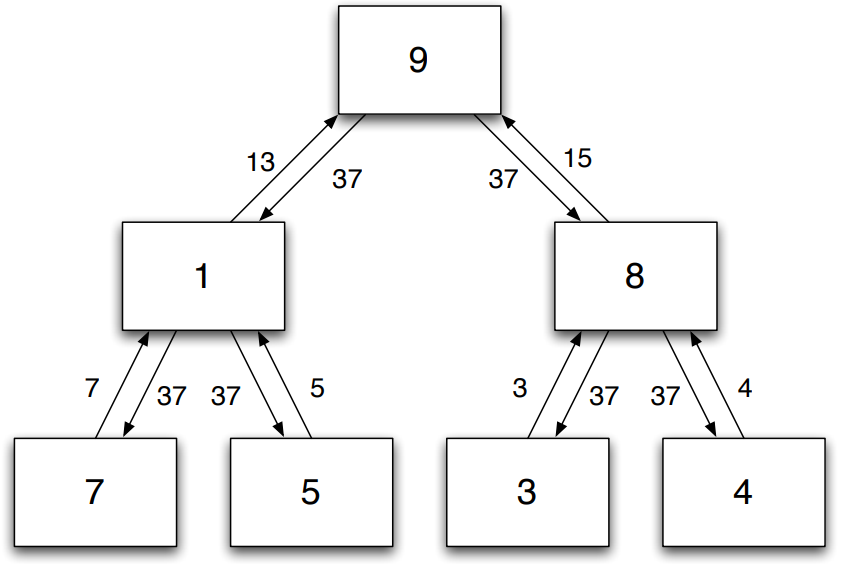
\includegraphics[scale=0.5]{AllReduce.png}
		\captionof{figure}{AllReduce operation. Initially, each node holds its own value. Values are passed up the tree and summed, until the global sum is obtained in the root node (reduce phase). The global sum is then passed back down to all other nodes (broadcast	phase). At the end, each node contains the global sum.}
	\end{minipage}
	\item \textbf{Centralized storage} Centralized storage is used for topologies where a single "master" or "server" node is in the center and many "slave" or "client" nodes communicate only with this master node. A practical implementation of this is the Parameter Server paradigm (PS). Each parameter server keeps a shard of the global model parameters as a key-value store. Each client communicates with the parameter server to read / update the parameters. \\
	An advantage is that all model parameters are in a global shared memory which makes it easy to inspect the model. A disadvantage is that the parameter servers are a bottleneck because they're handling all communication. To partly accommodate this issue, the techniques mentioned under "Bridging computation and communication" are used.
	\item \textbf{Decentralized storage} In contrast to centralized storage, in decentralized storage every worker maintains its own local view of the parameters and the workers communicate directly to each other. An example implementation is a peer-to-peer network where every machine broadcasts everything to all other machines. To reduce the amount of communication between all workers, Sufficient Factor Broadcasting (SFB)\cite{Li13}) was proposed. It Decomposes the parameter matrix \textbf{W} into the outer products of the two vectors \textbf{u} and \textbf{v}: \textbf{ΔW = uv\textsuperscript{T}}. The vectors u and v are \textit{sufficient factors}, meaning that they are sufficient to reconstruct the update matrix \textbf{ΔW}. SFB only broadcasts the sufficient factors and lets the workers reconstruct the updates.\\
	An advantage is that, with SFB, decentralized storage is relatively communication efficient and that there is no centralized bottleneck, making it more scalable.
\end{itemize}










\subsection{Currently used implementations}
\subsubsection{Generic distributed system frameworks}
\subsubsection{Domain-specific implementations}
\subsubsection{Current challenges}










\subsection{Privacy challenges}
